\documentclass[11pt]{article}
\usepackage{pgfplots}
\usetikzlibrary{patterns}
\usepackage{amssymb}
\usepackage{amsmath}
\usepgfplotslibrary{dateplot}
\usepackage[T1]{fontenc}
\usepackage[utf8]{inputenc}

\begin{document}

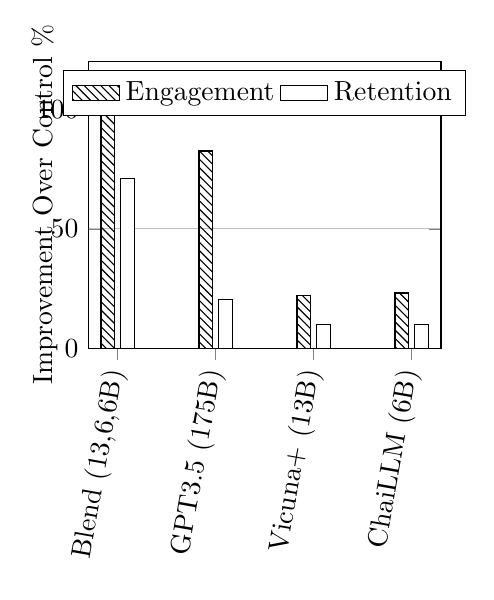
\begin{tikzpicture}
    \begin{axis}
        [
            ybar,
            bar width=5pt,
            legend style={at={(0.5, 0.97)},
            anchor=north,legend columns=-1},
            ylabel={Improvement Over Control \%},
            ylabel style={yshift=-10pt, inner sep=-1pt},
            symbolic x coords={1,2,3,4},
            xtick=data,
            xticklabels={{Blend (13,6,6B)}, GPT3.5 (175B), Vicuna+ (13B), ChaiLLM (6B)},
            xticklabel style={rotate=80, anchor=east},
            xtick pos=left,
            ymajorgrids=true,
            width=0.5\textwidth,
            ymin=0,
            ymax=120,
        ]
        \addplot[pattern=north west lines, pattern color=black, area legend] coordinates {(1, 110) (2, 82.5) (3, 22) (4, 23.2)};
        \addplot[fill=white, area legend] coordinates {(1, 71.2) (2, 20.5) (3, 10.2) (4, 10.1)};
        \legend{Engagement,Retention}
    \end{axis}
\end{tikzpicture}

\end{document}